\documentclass[11pt,twocolumn]{article}
\usepackage[T1]{fontenc}
\usepackage[
  paperwidth=21.9cm,
  paperheight=27.6cm,
  margin=1in,
  marginparwidth=0.8in,
  marginparsep=0.2in
]{geometry}
\usepackage{amsmath}
\usepackage{mathtools}
\usepackage{siunitx}
\usepackage{marginnote}
\usepackage{physics}
\usepackage{pdfpages}

% Links
\usepackage{hyperref}
\hypersetup{
  colorlinks=true,
  linkcolor=blue,
  urlcolor=cyan,
}

\usepackage{tikz}

% For \wavyseparator
\usetikzlibrary{decorations.pathmorphing}

% For magnetic field diagrams
\usetikzlibrary{angles,quotes} % for pic (angle labels)
\usetikzlibrary{calc}
\usetikzlibrary{decorations.markings}
\tikzset{>=latex} % for LaTeX arrow head

% For arrow note
\usetikzlibrary{tikzmark,positioning}

% Command for adding notes in the margin depending on single or double column layout
\makeatletter
\newcommand{\columnnote}[1]{%
  \if@twocolumn
  \if@firstcolumn
  \reversemarginpar
  \marginnote{\small\emph{#1}}%
  \normalmarginpar
  \else
  \normalmarginpar
  \marginnote{\small\emph{#1}}%
  \fi
  \else
  \marginnote{\small\emph{#1}}%
  \fi
}
\makeatother

\colorlet{Bcol}{violet!90}
\colorlet{BFcol}{red!60!black}
\colorlet{veccol}{green!45!black}
\colorlet{Icol}{blue!70!black}
\tikzstyle{BField}=[->,very thick,Bcol]
\tikzstyle{current}=[->,Icol] %thick,
\tikzstyle{force}=[->,very thick,BFcol]
\tikzstyle{velocity}=[->,very thick,vcol]
\tikzstyle{charge+}=[very thin,draw=black,top color=red!50,bottom color=red!90!black,shading angle=20,circle,inner sep=0.5]
\tikzstyle{charge-}=[very thin,draw=black,top color=blue!50,bottom color=blue!80,shading angle=20,circle,inner sep=0.5]
\tikzstyle{vector}=[->,thick,veccol]
\tikzset{
  BFieldLine/.style={thick,Bcol,decoration={markings,mark=at position #1 with {\arrow{latex}}},
  postaction={decorate}},
  BFieldLine/.default=0.5,
  pics/Bin/.style={
    code={
      \def\R{0.12}
      \draw[pic actions,Bcol,line width=0.6] % ,thick
      (0,0) circle (\R) (-135:.7*\R) -- (45:.7*\R) (-45:.7*\R) -- (135:.7*\R);
  }},
}

\newcommand{\wavyseparator}{%
  \par\vspace{0.5\baselineskip}%
  \noindent\centerline{\tikz{\draw[decorate, decoration={snake, amplitude=1mm, segment length=10mm}]
  (0,0) -- (0.8\linewidth,0);}}%
  \vspace{0.75\baselineskip}\par
}

% Make subsection counters alphabetic like in the textbook
\renewcommand\thesubsection{\thesection\Alph{subsection}}

% Customise subsection titles to show textbook page number in margin
\newcommand\mysubsection[2]{\subsection[#1]{#1\protect\columnnote{Textbook page \hyperlink{page.\number\numexpr#2+12\relax}{#2}}}}

% document metadata
\title{Pearson Edexcel International A Level Physics 2 - Notes}
% \author{Course: \underline{\hspace{5cm}} \quad Instructor: \underline{\hspace{5cm}}}
\date{\today}

\begin{document}
% \maketitle
% \tableofcontents
\bigskip

\setcounter{section}{5}
\section{Electric and Magnetic Fields}
\setcounter{subsection}{2}
\mysubsection{Electromagnetic Effects}{56}

Gravitational, electric and magnetic fields are all vector fields. The strength of each field is defined as the force per unit something experienced by an object placed in the field:

\[
  \begin{alignedat}{3}
    \vec g                        &= \frac{\vec F} m &\qquad
    \vec E                        &= \frac{\vec F} q &\qquad
    \vec B                        &= \frac{\vec F}{q \vec v} \\[1em]
    \tikzmarknode{phiVgrav}{\Phi} &= \frac W m        &
    V                             &= \frac W q        &
    ?                             &= \frac W {q \vec v}
  \end{alignedat}
\]

\begin{tikzpicture}[remember picture, overlay]
  \node[
    font=\footnotesize
  ] (note) at ([xshift=-2em,yshift=-2em]phiVgrav)
  {Or $V_\text{grav}$};
  \draw[->, semithick] (note.north) -- (phiVgrav.south west);
\end{tikzpicture}

\wavyseparator

\[
  \begin{aligned}
    W &= \vec F \cdot \vec s \\
    W &= \abs*{\vec F}\abs*{\vec s}\cos\theta
  \end{aligned}
\]

\wavyseparator

Magnetic fields can cause circular motion!

\begin{center}
  % Adapted from https://tikz.net/magnetic_field/ by Izaak Neutelings

% B FIELD horizontal, top view, circle
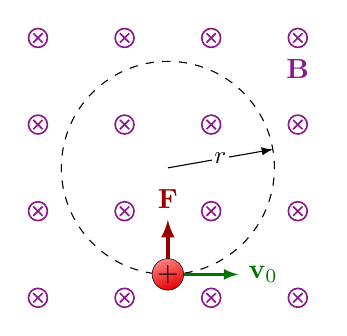
\begin{tikzpicture}
  \def\xmax{3.3}
  \def\ymax{3.3}
  \def\R{0.2}
  \def\P{0.41*\xmax}
  \def\v{0.21*\xmax}
  \def\F{0.15*\xmax}
  \def\NBy{4}
  \def\NBx{4}
  \coordinate (O) at (0.5*\xmax,0.09*\ymax+\P);
  \coordinate (Q) at (0.5*\xmax,0.09*\ymax);

  % Magnetic field
  \foreach \i [evaluate={\y=(\i-1)*\ymax/(\NBy-1);}] in {1,...,\NBy}{
    \foreach \i [evaluate={\x=(\i-1)*\xmax/(\NBx-1);}] in {1,...,\NBx}{
      \pic[rotate=-90] at (\x,\y) {Bin};
    }
  }
  \node[Bcol] at (\xmax,0.88*\ymax) {$\vb{B}$};

  % Charge
  \draw[dashed] (Q) arc (-90:270:\P) coordinate (F);
  \draw[vector] (Q)++(\R,0) --++ (\v,0) node[right] {$\vb{v}_0$};
  \draw[force]  (Q)++(0,\R) --++ (0,\F) node[above=0] {$\vb{F}$};
  \draw[charge+] (Q) circle (\R) node {$+$};
  \draw[->] (O) --++ (10:\P) node[midway,fill=white,inner sep=1,scale=0.9] {$r$};
\end{tikzpicture}

\end{center}

The forces involved are the magnetic force and the centripetal force:

\[
  \begin{alignedat}{2}
    \vec F_B &= q \vec v \cdot \vec B &\qquad
    \vec F_{cr} &= \frac{m \vec{v}^{\,2}} r
  \end{alignedat}
\]

Equating the magnetic force to the centripetal force, we can solve for the radius of the circular path:

\[
  \begin{aligned}
    q \vec v \cdot \vec B &= \frac{m \vec{v}^{\,2}} r \\
    q \vec B &= \frac{m \vec v} r \\
    r &= \frac{m \vec v}{q \vec B} \\
    r &= \frac{\vec p}{q \vec B}
  \end{aligned}
\]

\paragraph{See also}
\begin{itemize}
  \item
    Raycast AI Chat, Gemini 2.5 Pro: \href{raycast://extensions/raycast/raycast-ai/ai-chat?context=%7B%22id%22:%221D3C7992-8470-4794-9406-353F68D5E439%22%7D}{%
      Electromagnetic Induction and Magnetic Forces: Equations, hints, and problem-solving
    }
\end{itemize}

\wavyseparator

Magnetic flux through an area $A$ in a magnetic field $B$ is given by:

\[
  \begin{aligned}
    \Phi &= \vec B \cdot \vec A \\
    \Phi &= \abs*{\vec B}\abs*{\vec A}\cos\theta
  \end{aligned}
\]

Where $\Phi$ is in \href{https://wikipedia.org/wiki/Weber_(unit)}{webers}, \unit{\weber}, or \si{\tesla\metre\squared}, since $B$ is in \href{https://wikipedia.org/wiki/Tesla_(unit)}{teslas} and $A$ is in square metres.

\wavyseparator

More magnetic flux stuff:

\[
  \begin{aligned}
    \dv t \Phi &= V \\
    \dv t N\Phi &= V
  \end{aligned}
\]

\begin{quote}
  The rate of change of flux linkage through a coil gives the induced e.m.f. across the coil.
\end{quote}

\begin{center}
  % B FIELD horizontal, top view, circle
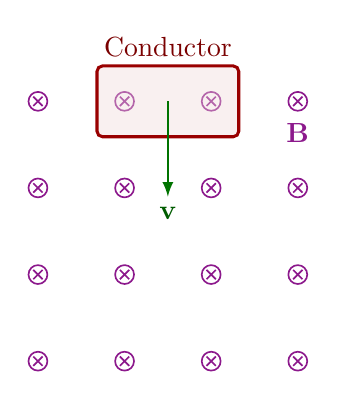
\begin{tikzpicture}
  \def\xmax{3.3}
  \def\ymax{3.3}
  \def\NBy{4}
  \def\NBx{4}

  \pgfmathsetmacro{\xstep}{\xmax/(\NBx-1)}
  \pgfmathsetmacro{\ystep}{\ymax/(\NBy-1)}

  % Magnetic field
  \foreach \i [evaluate={\y=(\i-1)*\ymax/(\NBy-1);}] in {1,...,\NBy}{
    \foreach \i [evaluate={\x=(\i-1)*\xmax/(\NBx-1);}] in {1,...,\NBx}{
      \pic[rotate=-90] at (\x,\y) {Bin};
    }
  }
  \node[Bcol] at (\xmax,0.88*\ymax) {$\vb{B}$};

  % Conductor: rectangle, positioned so it contains the top center two B field into-the-page symbols
  \coordinate (BmidL) at (\xstep, \ymax);
  \coordinate (BmidR) at (2*\xstep, \ymax);
  \def\padx{0.35}
  \def\pady{0.45}

  \draw[draw=BFcol, fill=BFcol!15, fill opacity=0.4, line width=1.1pt, rounded corners=2pt]
  ($(BmidL)+(-\padx,-\pady)$)
  rectangle
  ($(BmidR)+(\padx,\pady)$);

  \node[anchor=south, BFcol!80!black]
  at ($(BmidL)!0.5!(BmidR)+(0,\pady)$) {Conductor};

  % Motion arrow
  \draw[vector]
  ($(BmidL)!0.5!(BmidR)$)
  -- ++(0,-1.1*\ystep)
  node[below, veccol!80!black] {$\vb{v}$};
\end{tikzpicture}

\end{center}

Or we can have induction with a rotating coil in a magnetic field:

\begin{center}
  TODO: diagram
\end{center}

Here, e.m.f. is given by:

\[
  \begin{aligned}
    V &= \dv t [N\Phi] \\
    V &= N \dv{\Phi}{t} \\
    V &= N \dv t (\vec B \cdot \vec A) \\
    V &= N \dv t (\abs*{\vec B}\abs*{\vec A}\cos\theta)
  \end{aligned}
\]

Using $A = \abs*{\vec A}$ and $B = \abs*{\vec B}$ for simplicity:

\[
  \begin{aligned}
    V &= NBA \dv t [\cos\theta] \\
    V &= NBA \dv t [\cos\omega t] \\
    V &= -NBA \omega \sin(\omega t)
  \end{aligned}
\]

% https://steeven9.github.io/USI-LaTeX/html/math_graph.html
% https://tex.stackexchange.com/a/253040

\clearpage
\onecolumn
% \includepdf[pages=-]{textbook.pdf}

\end{document}
